\chapter{Internet of Things}
This chapter provides an overview of NB-IoT technology and its competitors. First, we will describe the NB-IoT technology in detail, including its architecture, physical layer, and protocol stack. Then, we will discuss the competitive landscape by comparing NB-IoT to other LPWA technologies such as Sigfox, LoRaWAN, and LTE Cat-M.

\section{NB-IoT Technology Overview}
NB-IoT is a cellular technology designed to provide wide-area coverage for IoT devices. It is based on the LTE standard and operates in the licensed spectrum. NB-IoT is a part of the 3GPP Release 13 specification, which was finalized in June 2016. The first commercial NB-IoT networks were launched in 2017, and the technology has been steadily gaining traction ever since \cite{ubox}.

\begin{figure}[h]
    \centering
    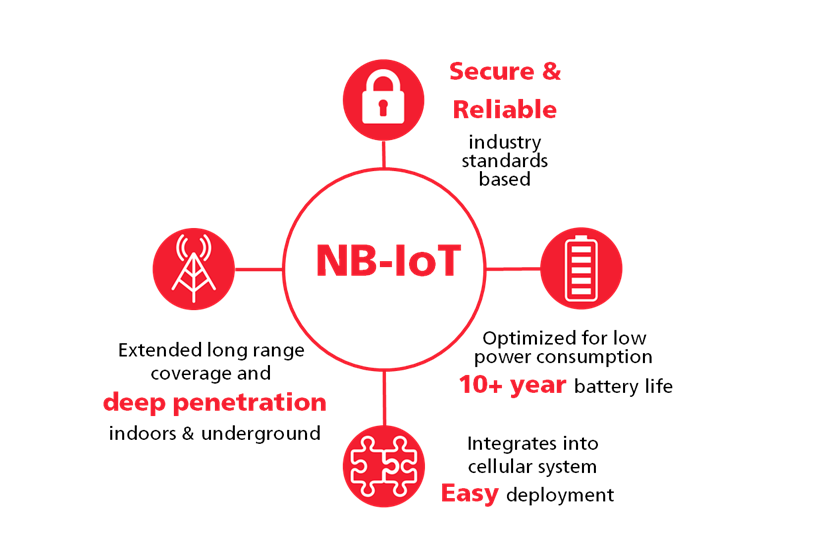
\includegraphics[width=0.8\textwidth]{pict/nb-iot.png}
    \caption{Features of NB-IoT \cite{ubox}}
    \label{fig:features-of-nb_iot}
\end{figure}

\subsection{NB-IoT Architecture}
The NB-IoT architecture is based on the LTE architecture, with some modifications to reduce the complexity and cost of the devices. The main components of the NB-IoT architecture are the user equipment (UE), evolved NodeB (eNB), and the core network (CN). The UE is the device that communicates with the network, while the eNB is the base station that provides the radio access network (RAN). The CN is responsible for the control and management of the network. The NB-IoT architecture is shown in Figure \ref{fig:nb-iot-architecture}.
\begin{figure}[ht]
    \centering
    \includegraphics[width=0.8\textwidth]{figures/nb-iot-architecture.png}
    \caption{NB-IoT architecture \cite{nb-iot-architecture}}
    \label{fig:nb-iot-architecture}
\end{figure}

\subsection{NB-IoT Physical Layer}
The NB-IoT physical layer is based on the LTE physical layer. It uses the same OFDM modulation scheme and subcarrier spacing as LTE. However, it uses a narrower bandwidth of 180 kHz, compared to 1.4 MHz in LTE. The NB-IoT physical layer also uses a different cyclic prefix length and a different number of resource blocks. The NB-IoT physical layer parameters are shown in Table \ref{tab:nb-iot-physical-layer}.
\begin{table}[ht]
    \centering
    \begin{tabular}{|l|l|}
        \hline
        \textbf{Parameter} & \textbf{Value} \\ \hline
        Modulation & QPSK \\ \hline
        Subcarrier spacing & 15 kHz \\ \hline
        Cyclic prefix length & Normal \\ \hline
        Number of resource blocks & 6 \\ \hline
        Bandwidth & 180 kHz \\ \hline
    \end{tabular}
    \caption{NB-IoT physical layer parameters \cite{nb-iot-physical-layer}}
    \label{tab:nb-iot-physical-layer}
\end{table}

\subsection{NB-IoT Protocol Stack}
The NB-IoT protocol stack is based on the LTE protocol stack. It uses the same radio resource control (RRC) protocol, as well as the same packet data convergence protocol (PDCP) and radio link control (RLC) protocol. However, it uses a different medium access control (MAC) protocol and physical layer. The NB-IoT protocol stack is shown in Figure \ref{fig:nb-iot-protocol-stack}.
\begin{figure}[Ht]
    \centering
    \includegraphics[width=0.8\textwidth]{figures/nb-iot-protocol-stack.png}
    \caption{NB-IoT protocol stack \cite{nb-iot-protocol-stack}}
    \label{fig:nb-iot-protocol-stack}
\end{figure}

\subsection{NB-IoT Releases}
The NB-IoT standard has been evolving since its initial release in 2016. The first release, Release 13, was finalized in June 2016. It was followed by Release 14 in June 2017 and Release 15 in June 2018. The latest release, Release 16, was finalized in July 2020. The NB-IoT releases are shown in Table \ref{tab:nb-iot-releases}.
\begin{table}[ht]
    \centering
    \begin{tabular}{|l|l|}
        \hline
        \textbf{Release} & \textbf{Date} \\ \hline
        Release 13 & June 2016 \\ \hline
        Release 14 & June 2017 \\ \hline
        Release 15 & June 2018 \\ \hline
        Release 16 & July 2020 \\ \hline
    \end{tabular}
    \caption{NB-IoT releases \cite{nb-iot-releases}}
    \label{tab:nb-iot-releases}
\end{table}

\subsubsection{Release 13}
Release 13 was the first release of NB-IoT. It introduced the initial set of features, including the physical layer, protocol stack, and architecture. It also defined the maximum transmission power, maximum number of repetitions, and maximum number of repetitions per PRB. The maximum transmission power was set to 20 dBm, while the maximum number of repetitions was set to 2048. The maximum number of repetitions per PRB was set to 4.

\subsubsection{Release 14}
Release 14 introduced several new features, including the support for multi-tone transmissions, the support for multi-tone reception, and the support for multi-tone reception with multiple antennas. It also introduced the support for multi-tone transmission with multiple antennas. The maximum number of repetitions was increased to 4096, while the maximum number of repetitions per PRB was increased to 8.

\subsubsection{Release 15}
Release 15 introduced several new features, including the support for multi-tone transmission with multiple antennas, the support for multi-tone reception with multiple antennas, and the support for multi-tone reception with multiple antennas and multiple PRBs. It also introduced the support for multi-tone transmission with multiple antennas and multiple PRBs. The maximum number of repetitions was increased to 8192, while the maximum number of repetitions per PRB was increased to 16.

\subsubsection{Release 16}
Release 16 introduced several new features, including the support for multi-tone transmission with multiple antennas and multiple PRBs, the support for multi-tone reception with multiple antennas and multiple PRBs, and the support for multi-tone reception with multiple antennas and multiple PRBs and multiple PRBs. It also introduced the support for multi-tone transmission with multiple antennas and multiple PRBs and multiple PRBs. The maximum number of repetitions was increased to 16384, while the maximum number of repetitions per PRB was increased to 32.

\subsection{NB-IoT Deployment Modes}
NB-IoT supports three deployment modes: in-band, guard-band, and standalone. In-band deployment uses the same spectrum as LTE, while guard-band deployment uses the guard-band between LTE and GSM. Standalone deployment uses the GSM spectrum. The NB-IoT deployment modes are shown in Figure \ref{fig:nb-iot-deployment-modes}.
\begin{figure}[ht]
    \centering
    \includegraphics[width=0.8\textwidth]{figures/nb-iot-deployment-modes.png}
    \caption{NB-IoT deployment modes \cite{nb-iot-deployment-modes}}
    \label{fig:nb-iot-deployment-modes}
\end{figure}

\subsection{NB-IoT Frequency Bands}
NB-IoT supports several frequency bands, including 450 MHz, 700 MHz, 800 MHz, 850 MHz, 900 MHz, 1800 MHz, 1900 MHz, 2100 MHz, and 2600 MHz. The NB-IoT frequency bands are shown in Table \ref{tab:nb-iot-frequency-bands}.
\begin{table}[ht]
    \centering
    \begin{tabular}{|l|l|}
        \hline
        \textbf{Frequency Band} & \textbf{Bandwidth} \\ \hline
        450 MHz & 1.4 MHz \\ \hline
        700 MHz & 1.4 MHz \\ \hline
        800 MHz & 200 kHz \\ \hline
        850 MHz & 200 kHz \\ \hline
        900 MHz & 200 kHz \\ \hline
        1800 MHz & 200 kHz \\ \hline
        1900 MHz & 200 kHz \\ \hline
        2100 MHz & 200 kHz \\ \hline
        2600 MHz & 200 kHz \\ \hline
    \end{tabular}
    \caption{NB-IoT frequency bands \cite{nb-iot-frequency-bands}}
    \label{tab:nb-iot-frequency-bands}
\end{table}

\subsection{NB-IoT Maximum Transmission Power}
NB-IoT power class defines the maximum transmission power of the device. It is defined in dBm and ranges from 20 dBm to 23 dBm. The NB-IoT power classes are shown in Table \ref{tab:nb-iot-power-classes}.

\begin{table}[ht]
    \centering
    \begin{tabular}{|l|l|}
        \hline
        \textbf{Power Class} & \textbf{Maximum Transmission Power} \\ \hline
        Power Class 1 & 20 dBm \\ \hline
        Power Class 2 & 21 dBm \\ \hline
        Power Class 3 & 22 dBm \\ \hline
        Power Class 4 & 23 dBm \\ \hline
    \end{tabular}
    \caption{NB-IoT power classes \cite{nb-iot-power-classes}}
    \label{tab:nb-iot-power-classes}
\end{table}

\subsection{NB-IoT Maximum Number of Repetitions}
NB-IoT supports the transmission of multiple repetitions of the same message. The maximum number of repetitions is defined in the NB-IoT standard and ranges from 2048 to 16384. The NB-IoT maximum number of repetitions is shown in Table \ref{tab:nb-iot-maximum-number-of-repetitions}.
\begin{table}[ht]
    \centering
    \begin{tabular}{|l|l|}
        \hline
        \textbf{Release} & \textbf{Maximum Number of Repetitions} \\ \hline
        Release 13 & 2048 \\ \hline
        Release 14 & 4096 \\ \hline
        Release 15 & 8192 \\ \hline
        Release 16 & 16384 \\ \hline
    \end{tabular}
    \caption{NB-IoT maximum number of repetitions \cite{nb-iot-maximum-number-of-repetitions}}
    \label{tab:nb-iot-maximum-number-of-repetitions}
\end{table}

\subsection{NB-IoT Maximum Number of Repetitions per PRB}
NB-IoT supports the transmission of multiple repetitions of the same message per PRB. The maximum number of repetitions per PRB is defined in the NB-IoT standard and ranges from 4 to 32. The NB-IoT maximum number of repetitions per PRB is shown in Table \ref{tab:nb-iot-maximum-number-of-repetitions-per-prb}.  
\begin{table}[ht]
    \centering
    \begin{tabular}{|l|l|}
        \hline
        \textbf{Release} & \textbf{Maximum Number of Repetitions per PRB} \\ \hline
        Release 13 & 4 \\ \hline
        Release 14 & 8 \\ \hline
        Release 15 & 16 \\ \hline
        Release 16 & 32 \\ \hline
    \end{tabular}
    \caption{NB-IoT maximum number of repetitions per PRB \cite{nb-iot-maximum-number-of-repetitions-per-prb}}
    \label{tab:nb-iot-maximum-number-of-repetitions-per-prb}    
\end{table}

\subsection{NB-IoT Maximum Number of Repetitions per PRB per Subframe}
NB-IoT supports the transmission of multiple repetitions of the same message per PRB per subframe. The maximum number of repetitions per PRB per subframe is defined in the NB-IoT standard and ranges from 1 to 4. The NB-IoT maximum number of repetitions per PRB per subframe is shown in Table \ref{tab:nb-iot-maximum-number-of-repetitions-per-prb-per-subframe}.
\begin{table}[ht]
    \centering
    \begin{tabular}{|l|l|}
        \hline
        \textbf{Release} & \textbf{Maximum Number of Repetitions per PRB per Subframe} \\ \hline
        Release 13 & 1 \\ \hline
        Release 14 & 2 \\ \hline
        Release 15 & 3 \\ \hline
        Release 16 & 4 \\ \hline
    \end{tabular}
    \caption{NB-IoT maximum number of repetitions per PRB per subframe \cite{nb-iot-maximum-number-of-repetitions-per-prb-per-subframe}}
    \label{tab:nb-iot-maximum-number-of-repetitions-per-prb-per-subframe}
\end{table}

\subsection{NB-IoT Maximum Number of Repetitions per PRB per Subframe per Antenna}
NB-IoT supports the transmission of multiple repetitions of the same message per PRB per subframe per antenna. The maximum number of repetitions per PRB per subframe per antenna is defined in the NB-IoT standard and ranges from 1 to 4. The NB-IoT maximum number of repetitions per PRB per subframe per antenna is shown in Table \ref{tab:nb-iot-maximum-number-of-repetitions-per-prb-per-subframe-per-antenna}.

\begin{table}[ht]
    \centering
    \begin{tabular}{|l|l|}
        \hline
        \textbf{Release} & \textbf{Maximum Number of Repetitions per PRB per Subframe per Antenna} \\ \hline
        Release 13 & 1 \\ \hline
        Release 14 & 2 \\ \hline
        Release 15 & 3 \\ \hline
        Release 16 & 4 \\ \hline
    \end{tabular}
    \caption{NB-IoT maximum number of repetitions per PRB per subframe per antenna \cite{nb-iot-maximum-number-of-repetitions-per-prb-per-subframe-per-antenna}}
    \label{tab:nb-iot-maximum-number-of-repetitions-per-prb-per-subframe-per-antenna}
\end{table}

\subsection{NB-IoT Maximum Number of Repetitions per PRB per Subframe per Antenna per Antenna}
